%!TEX root = ../Main.tex
The Green's function and self energies play the central role when it comes to obtaining the LDOS as well as electron transport in a system. In fact, the imaginary part of the Green's function is the LDOS for a specific site in a system. What the Green's function and self energy actually is and how they come about will here be explained formally, to motivate the practical use in the following sections.\subsection{Green's functions and selfenergy}\label{greensandself} 
Firstly on should note that some of the concepts in this section will be explained using a figure of NPG as an example (\cref{atomrepfig}). However, in the following section (\cref{recursionroutinesec}) the focus will revert back to the simple system from \cref{pointplot}. \begin{figure}[H]
	\centering
	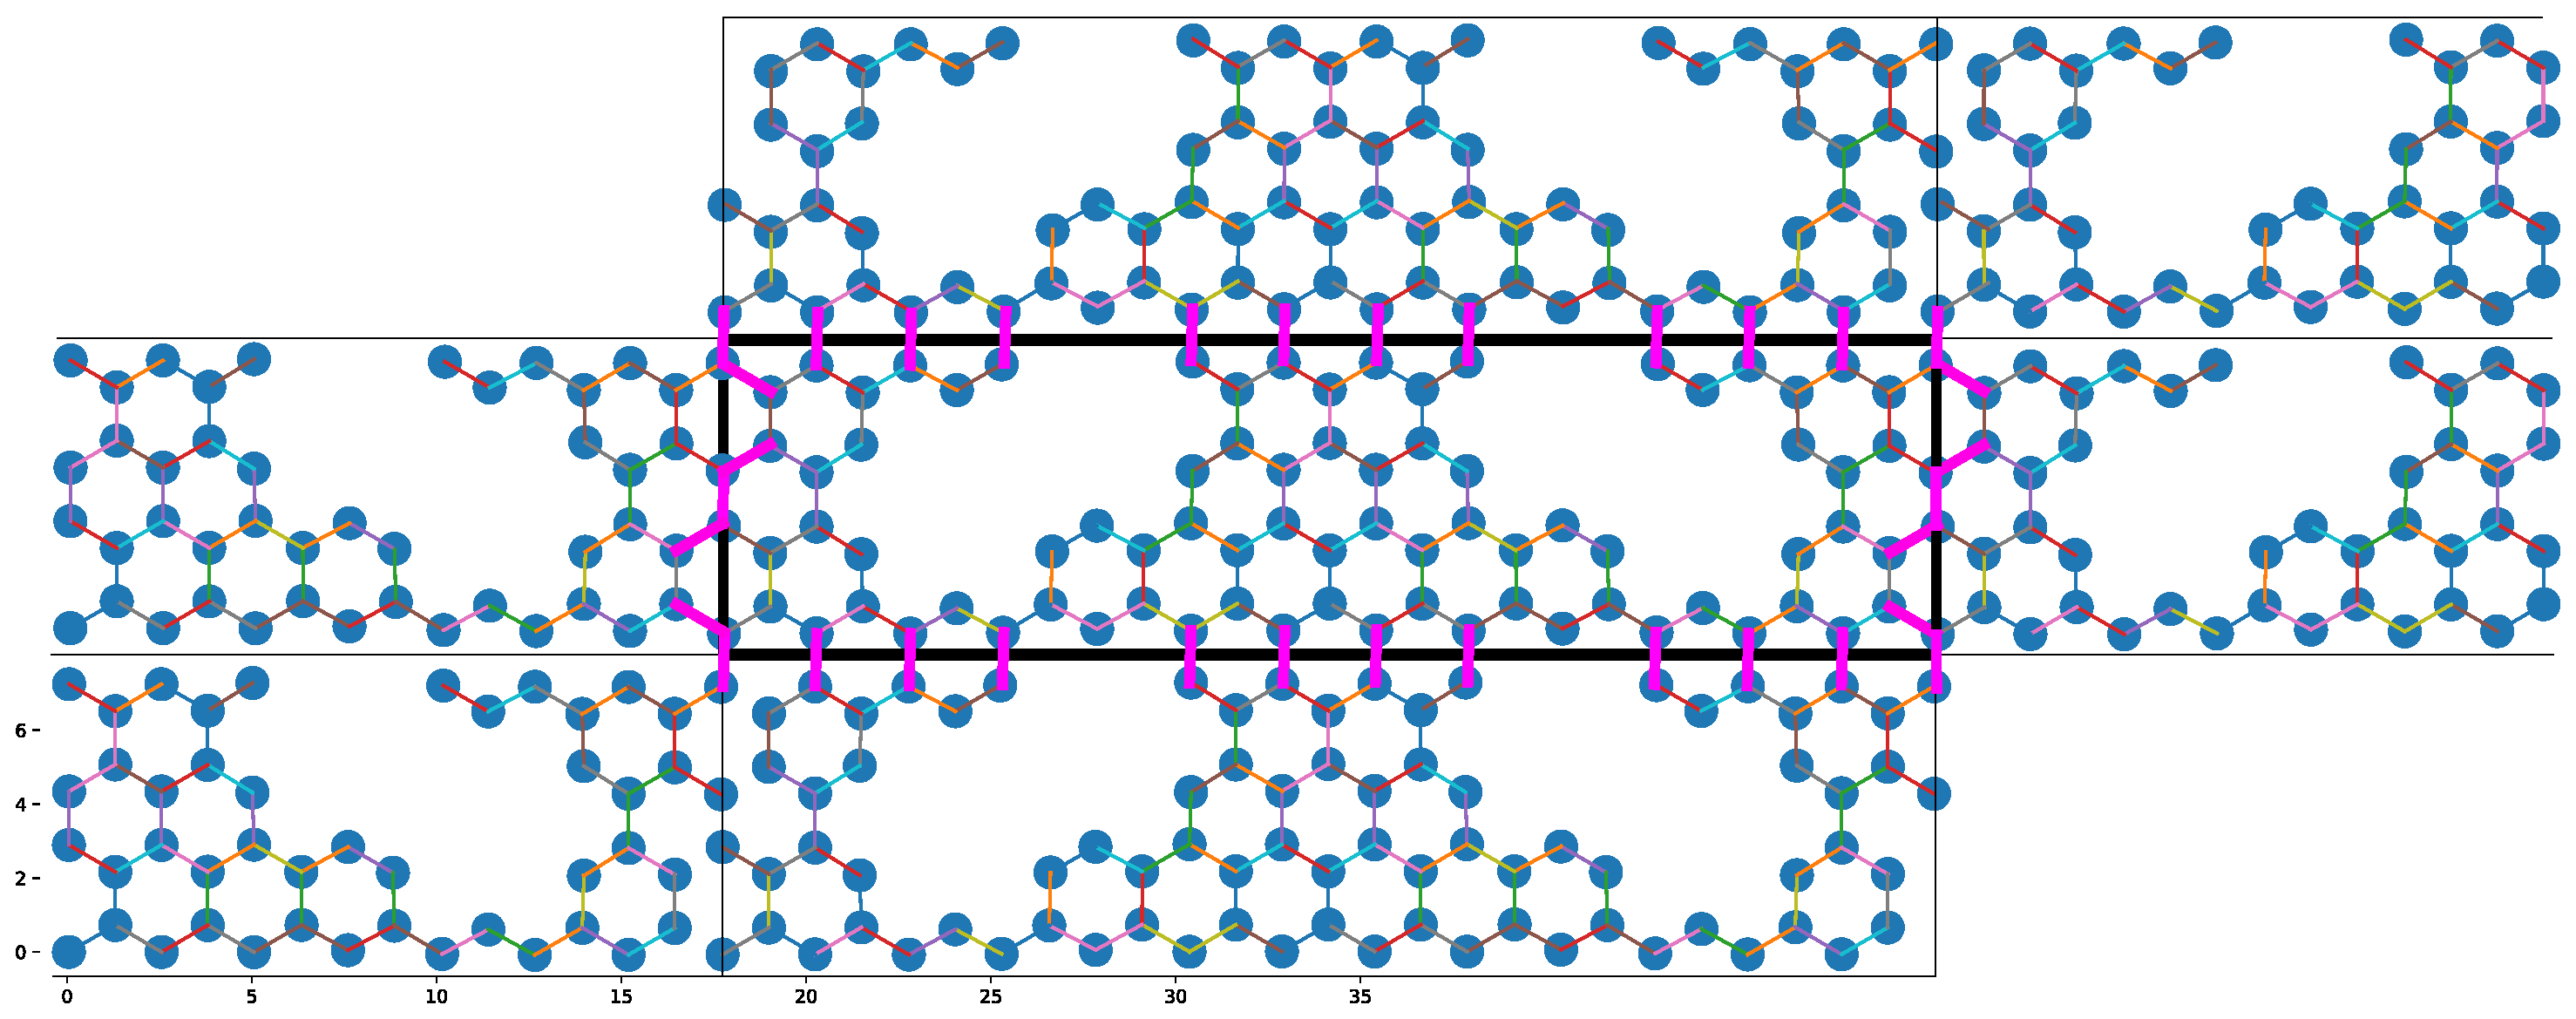
\includegraphics[width=\textwidth]{Figures/representativestructure2.eps}
	\caption{Visual representation of the periodic NPG-structure. The atoms surrounded by the black box in the centre represents the unit cell. The neighbouring boxes are unit cells repeated periodically. Note that the two cells left and right with respect to the centre cell has been cut in half for figure space. The pink lines crossing the black box represents the link between the nearest neighbours in the adjacent cell.}
	\label{atomrepfig}
\end{figure}
%\begin{align}
%\mathbf{H}\phi(t) &= i\pdv{t}\phi(t) \\
%\mathbf{H}\mathbf{G}(t) &= i\pdv{t}\mathbf{G}(t)
%\end{align}
%with specific boundary conditions, namely\begin{align}\label{boundary}
%    \phi(t=0) = f 
%\end{align}
%The Green's function has the additional property that \(\mathbf{G}(t=0)=\mathbf{1}\) which means the one can solve the TDSE for any initial value of \(t\)  if one has solved the equation for the Green's function first.\begin{align}\label{greenssolution}
%    \phi(t)=\mathbf{G}(t)f
%\end{align}
%From \cref{greenssolution} it can be seen that the Green's function propagates the value \(f\) at \(t=0\). Now, if the Hamiltonian is time independent one can also consider time independent solutions to the Schr\"{o}dinger Equation. All states will then be oscillating with the same complex phase, at a specific energy \(E\). This will be given by \(e^{-iEt}\). 
Imagine a system like the one in \cref{atomrepfig}. It contains a unit cell in the centre, marked by a black border, surrounded by repeated unit cells in all directions. The aim is to explain how electrons move through this region. Suppose all cells surrounding the centre cell are considered "contacts" in the sense that they represent a semi-infinite chain of molecules and that they are the source of electrons (or states) that is injected in to the centre cell. What the Green's function is doing is that it "takes the states through" the centre region. It propagates the states in this particular area. In other words, the Green's function is the solution to the Schr\"{o}dinger Equation in this area and the equation has the form 
\begin{align}\label{Greensunsolved}
    [(E+i\eta)\mathbf{1}-\mathbf{H}]\mathbf{G}(E) = \mathbf{1}
\end{align}
From this equation one can also get the Green's function as 
\begin{align}\label{Greenssolved}
    \mathbf{G}(E) &= \mathbf{1}([(E+i\eta)\mathbf{1}-\mathbf{H}])^{-1}\\
    & = [(E+i\eta)\mathbf{1}-\mathbf{H}]^{-1}
\end{align}
The Green's functions in these equations are represented as matrices that contain all the individual Green's functions for the unit cell as well a the Green's functions for the rest of the chain. As seen in the equations, all that is needed to get the Green's function for a unit cell, in theory, is an energy and the Hamiltonian of the unit cell. Note that the solution to the Green's function matrix is a diagonal matrix with the two first off diagonals because of rules for nearest neighbour interaction dictated by the Thigh Binding approximation. As the Green's functions for the all unit cells in a potentially semi-infinite system are needed, in practice, one has to turn to more sophisticated methods to obtain all the Green's functions, namely recursion. More on that shortly. For now this is the introduction to the Green's function. How it relates to a unit cell in a system and that it is the source of the LDOS in a unit cell.\\
As described  one can use the Green's functions to get the propagation of states through a specific on-site Hamiltonian. However, if the system contains a range of cells, possibly infinitely many, the Hamiltonian would be of infinite size and the inversion in \cref{Greenssolved} would be impossible to do practically. The solution to this, is to model a semi-infinite tight binding chain of atom/molecules and then use \textit{recursion} on this chain. The way the recursion is done is to remove every second cell in the chain. Because the chain is semi-infinite, the yield would just be a new semi-infinite chain. Continuing this way the system can be reduced to a finite size which can actually be worked on. Say one continues to remove every second element in the chain, then in the end, the cells would be too far apart to interact an no hopping between cells would occur. At this point the recursion should stop. More on how this is done practically later.  For now one just have to keep in mind that the removing cells in the chain effectively changes to coupling between them and this is where \textit{self energy} comes in. The self energy is what describes the effective coupling between a cell and the rest of the semi-infinite chain. And it can be derived by looking at a cell at the very end of the semi-infinite chain and see how it couples to the rest. First one needs the Green's functions. The Green's matrix for this single cell would be given by the equation in \cref{Greenssolved}. This is before when only one cell and thus one matrix had to be considered. But now, there is an semi-infinite amount of cells and an semi-infinite amount of matrices to consider. However, the cell in the end of the chain only interacts with the cell next to it and so on. Considering this one can write op an equation equivalent to that of \cref{Greensunsolved} but as system of matrix equations for the chain.
\begin{align}\label{Greenssystem}
\begin{pmatrix}
    z\mathbf{1}-\mathbf{H}_c & -\mathbf{V}^{\dagger} \\ -\mathbf{V} & (z-\varepsilon')\mathbf{1} 
\end{pmatrix}
\begin{pmatrix}
\mathbf{X} & \mathbf{G}_{0c}\\
\mathbf{G}_{c0} & \mathbf{G}_{00}
\end{pmatrix}
=
\begin{pmatrix}
\mathbf{1} & \mathbf{0} \\
\mathbf{0} & \mathbf{1}
\end{pmatrix}
\end{align}
where \(\varepsilon'\) is the on-site Hamiltonian of the first cell, \(z\) is \(E+i\eta\),  \(\mathbf{G}_{0c/c0}\) is the Green's matrices coupling the cell to the rest of the chain and \(\mathbf{X}\) is the Green's matrices for the rest of the chain. This is also assuming one knows the Green's function within the chain \(\mathbf{G}_c\) and that the chain has constant hopping and on-site elements \(\mathbf{H}_c,\mathbf{V},\mathbf{V}^{\dagger}\). 
Solving this system for \(\mathbf{G}_{00}\) and eliminating \(\mathbf{G}_{0c}\), which is unknown, one gets
\begin{align}\label{greenszero}
    \mathbf{G}_{00}(z) = (z-\varepsilon'-\Sigma(z))^{-1}
\end{align}
where \(\Sigma(z)\) is the self-energy. One can isolate the self energy from the equations above to
\begin{align}
    \mathbf{\Sigma}(z) = \mathbf{V}[z\mathbf{1}-\mathbf{H}_c]^{-1}\mathbf{V}^{\dagger}
\end{align}
And this concludes the formal introduction to Green's functions and self energy.\subsection{Obtaining first cell self-energy and Green's matrix  for the simple system through programming}\label{recursionroutinesec}
For simplicity and in order to check whether the routine would yield the expected results, the system in \cref{pointplot} is use as an example. The goal is to get the Green's functions for the centre unit cell in the semi-infinite chain and the self energies coupling to rest of the chain right and left. Specifically for the simple system one should imagine first having one centre unit cell like \cref{pointplot} and then repeating it infinitely in the left and right direction. The fact that there is a left \textit{and} right self energy is that the unit cell lies within the semi-infinite chain and not at the very end as described in \cref{greensandself}. To be assured, this does not conflict with any of the preciously mentioned formalism and the left and right self energies are quite easily obtained as one shall see shortly. As mentioned the goal is to get the Green's functions of a specific unit cell and the self energies related to it. If the Green's matrix \(\mathbf{G}\) represents the whole chain, then the equation of the whole system would be equivalent to that of \cref{Greensunsolved}. Considering the Green's functions for specific unit cell in question, it would correspond to one column in the system of equations, say the first. One can define the on-site Hamiltonian \(\mathbf{h}_0\) for the specific unit cell and its hopping matrices \(\mathbf{V},\mathbf{V}^{\dagger}\).  The two hopping matrices correspond to hopping left or right in the chain respectively. These can be obtained using the functions already developed in \cref{hamilsec}. Throughout this section they will be named \(a_0 = \mathbf{V}^{\dagger}, \ b_0 = \mathbf{V}, \ e_{s0} = \mathbf{h}_{s}\). The recursion is an iterative process and so the zero index indicates the starting point of the iterations and the \textit{s} index indicates that it is the Hamiltonian of the specific wanted cell. One can also define a Green's function for a single unit cell as \(g_0 = (z-e_{0})^{-1}\) just like \cref{Greensunsolved} where \(e_{0}=\mathbf{h}\) which is the on-site Hamiltonian of the other cells. With these elements a system of equations, similar to \cref{Greensunsolved} can be setup. The first difference being that the identity matrix is replaced by its first column, because the solution of interest is that one first column in the Green's matrix. The second is that the first element in the Hamiltonian matrix \(\mathbf{H}\) is related to the specific single unit cell \(\mathbf{h}_s\). Next a range of multiplications of the different elements stated so far will be shown, and afterwards it will be explained how these affect the system of equations to give recursion. The multiplications are:
\begin{align}\label{matmulrec}
	a_1     & = a_0 \times g_0 \times a_0                   \\ \nonumber
	b_1     & = b_0\times g_0\times b_0                   \\ \nonumber
	e_1     & = e_0 + a_0\times g_0\times b_0 + b_0\times g_0\times a_0 \\ \nonumber
	e_{1s} & = e1_{0s} + a_0\times g_0\times b_0          \\ \nonumber
	g_1     & = (z - e_1)^{-1}
\end{align}
These equations constitutes the first iteration in the recursion and they can be repeated indefinitely. In the matrix system of equations  these multiplications effectively shifts all elements in the matrix by one column and because the matrix is diagonal, it will leave the first column of the matrix empty. The column can then be removed and this is exactly what corresponds to removing a cell in the semi-infinite chain. Keeping on doing these multiplications, raising the index by +1 every time, one can move through reduce the system as a whole removing of columns (cells) in the system of equations. In the end one will obtain re-normalised Hamiltonians and hopping matrices which is then used to get the Green's functions and self energies through these simple equations: 
\begin{align}\label{outputs}
	\mathbf{\Sigma}_R & = e_s - h                   \\ \nonumber
	\mathbf{\Sigma}_L & = e - h - \mathbf{\Sigma}_R \\ \nonumber
	\mathbf{G00}      & = (z - e_s)^{-1}
\end{align}
Programming this recursion is fairly simple as all which is needed is a while loop which iterates over the equations in \cref{matmulrec} until a threshold has been reached. The threshold is determined by the value of the hopping matrix \(a_0\). As it reaches a value close to zero, there is no longer any effective interacting (hopping) between the cells because of removal of cells and the recursion should stop. 
In \cref{recurfunc} the code for the routine is shown. Line xx-xx is the listing of elements before iteration, xx-xx is the while loop with the equations from \cref{matmulrec}. Note that some intermediate multiplications are made f.ex. \textit{ag = a0 @ b0}. This is for run-time optimisation only. In  line xx-xx the iteration indexed 0 gets redifned so that it corresponds to the most recent iteration. Finally in xx-xx the definition of the outputs as per \cref{outputs} is stated.\im{Listings/Functions.py}{62}{89}
\vspace{-1\baselineskip}
\captionof{listing}{The while loop in the recursion routine. The matrix elements are overwritten with the new variables until the resulting matrix is small enough to diagonalise\label{recurfunc}}\vspace{\baselineskip}
This concludes how recursion works and how the first cell Green's function as well as the self-energies is obtained. 
\subsection{Plotting the real and imaginary part of the first cell Green's function}
One of the results possible to obtain via the recursion routine is the Green's function of the centre unit cell in relation to the rest of the chain. As mentioned the imaginary part of the elements Green's matrix is the LDOS of the different sites in the unit cell. With a relatively simple approach, the Green's matrix elements can be obtained as a function of energy, using a \textit{for loop}, looping over a range of energies which is then used as input in the \textit{RecursionRoutine} function (\cref{recurfunc}), see \cref{plotcode}:
\im{Listings/SelfEnergyByRecursion.py}{64}{68}
\vspace{-1\baselineskip}
\captionof{listing}{Code showing the loop which produces the complex Green's function (or y) values for a range of energies used in the plot.\label{plotcode}}\vspace{\baselineskip}
This gives information about the LDOS at a specific energy and place in space, namely a specific atom in the unit cell. The resulting plot for the simple system (atom index 0) can be seen in \cref{LDOSsimple}. As seen in the plot... Note that the plot only represents the LDOS for a specific site on the molecule and that they may change radically from site to site (see \cref{appfigs}, \cref{siteLDOSplot} for an example using the same system as \cref{pointplot}). The site can be changed by choosing another index in \cref{plotcode} line 68, which corresponds to the atom indices in \cref{pointplot}. 